\documentclass[aspectratio=169,11pt]{beamer}

\usetheme{Madrid}
\usecolortheme{default}
\setbeamertemplate{navigation symbols}{}
\usepackage[T1]{fontenc}
\usepackage{lmodern}
\usepackage{tikz}
\usepackage{booktabs,array,tabularx}
\usetikzlibrary{shapes.geometric,arrows.meta,positioning,fit,backgrounds,calc}

\definecolor{aitblue}{RGB}{20,60,120}
\setbeamercolor{palette primary}{bg=aitblue,fg=white}
\setbeamercolor{palette secondary}{bg=aitblue!85,fg=white}
\setbeamercolor{palette tertiary}{bg=aitblue!70,fg=white}
\setbeamercolor{structure}{fg=aitblue}
\setbeamercolor{title}{bg=aitblue,fg=white}
\setbeamercolor{frametitle}{bg=aitblue,fg=white}

\title[Resource-Aware Collaborative Cloud IDE]{Resource-Aware Collaborative Cloud IDE using Intelligent Optimization and Container Orchestration}
\author{BE Computer 2026--2027}
\institute[AIT]{Army Institute of Technology\\Savitribai Phule Pune University\\Computer Engineering}
\date{October 28, 2026}

\newcommand{\guide}{Prof.\ Yogita Hambir}

% ---------- TikZ styles ----------
\tikzset{
  box/.style={draw=aitblue,fill=white,rounded corners=2pt,minimum height=0.7cm,
              align=center,font=\scriptsize,inner sep=3pt,thick},
  opt/.style={box,fill=orange!15,draw=orange!70!black},
  k8s/.style={box,fill=cyan!12,draw=cyan!60!black},
  dock/.style={box,fill=blue!8,draw=blue!60},
  mon/.style={box,fill=green!12,draw=green!50!black},
  cli/.style={box,fill=gray!10,draw=gray!70},
  arr/.style={-{Stealth[length=2.2mm]},thick,aitblue},
  darr/.style={-{Stealth[length=2.2mm]},thick,dashed,red!60!black},
  layer/.style={draw=aitblue!60,dashed,rounded corners=4pt,inner sep=6pt},
  lbl/.style={font=\tiny\bfseries,text=aitblue,anchor=south west}
}

\tikzset{g/.style={draw=#1,dashed,thick,rounded corners=3pt,fill=#1!5}}

\begin{document}

% ---------------- 1. Title ----------------
\begin{frame}
  \titlepage
  \vspace{-0.5em}
  \begin{center}
    \small Under the guidance of \textbf{\guide}
  \end{center}
\end{frame}

% ---------------- 2. Contents ----------------
\begin{frame}{Contents}
  \begin{enumerate}
    \item Introduction
    \item Problem Statement
    \item Gaps in Present Study
    \item Proposed Methodologies
    \item Resource Utilization
    \item System Architecture
    \item Conclusion
  \end{enumerate}
\end{frame}

% ---------------- 3. Introduction ----------------
\begin{frame}{Introduction}
  \begin{itemize}
    \item Modern software development is rapidly shifting toward cloud-based environments, enabling remote access and collaboration.
    \item Existing collaborative IDE platforms face \alert{high latency}, \alert{synchronization conflicts}, and \alert{inefficient resource utilization}, especially under dynamic multi-user workloads.
    \item This project proposes a collaborative cloud IDE that integrates real-time programming with intelligent resource management.
    \item By leveraging containerization and orchestration, the system aims to achieve scalability, efficiency, and optimized performance.
  \end{itemize}
\end{frame}

% ---------------- 4. Problem Statement ----------------
\begin{frame}{Problem Statement}
  \begin{itemize}
    \setlength{\itemsep}{0.8em}
    \item Latency issues during real-time code synchronization
    \item Conflict handling complexity in multi-user editing
    \item Inefficient resource allocation, leading to wastage
    \item Lack of adaptive scaling mechanisms
    \item Poor handling of dynamic workloads and user spikes
  \end{itemize}
\end{frame}

% ---------------- 5. Research Gaps ----------------
\begin{frame}{Research Gaps}
  The present study identifies the following gaps:
  \begin{itemize}
    \item Lack of integration between real-time collaboration and resource optimization
    \item Limited use of intelligent scheduling algorithms in cloud IDEs
    \item Inefficient handling of multi-user synchronization at scale
    \item Absence of energy-aware and resource-aware execution models
    \item Dependency on static resource allocation strategies
    \item Limited automation in container lifecycle and workload management
  \end{itemize}
\end{frame}

% ---------------- 6. Literature table ----------------
\begin{frame}[shrink=6]{Research Gaps: Literature Survey}
  \tiny
  \renewcommand{\arraystretch}{1.25}
  \begin{tabularx}{\textwidth}{>{\raggedright\arraybackslash}p{3.1cm}c>{\raggedright\arraybackslash}X>{\raggedright\arraybackslash}X}
    \toprule
    \textbf{Paper} & \textbf{Year} & \textbf{Methodology} & \textbf{Gaps}\\
    \midrule
    Adaptive Resource Allocation for Workflow Containerization on Kubernetes (Shan et al.) & 2023 &
    MAPE-K based adaptive resource allocation (ARAS), Kubernetes workflow engine, dynamic vertical scaling &
    No energy optimization, no intelligent optimization algorithms (ACO/PSO), lacks prediction capability, high monitoring overhead\\
    \addlinespace
    A Hybrid Multi-Faceted Task Scheduling Algorithm for Cloud Computing Environment (Dubey \& Sharma) & 2023 &
    Hybrid metaheuristic combining PSO and ACO, simulation using CloudSim &
    Not implemented in Kubernetes/container environment, no real-time scaling, no energy-aware optimization, only simulation-based validation\\
    \addlinespace
    Adaptive Energy Optimization in Cloud Computing Through Containerization (Beena et al.) & 2025 &
    Integration of ACO, PSO and DVFS with Kubernetes, adaptive resource adjustment (ARAA), automated lifecycle management (ARKLM) &
    No ML-based prediction, limited proactive decision-making, lacks workload forecasting, scope for improved intelligent adaptability\\
    \bottomrule
  \end{tabularx}
\end{frame}

% ---------------- 7. Proposed Solution (flowchart) ----------------
\begin{frame}{Proposed Solution: Workflow}
  \centering
  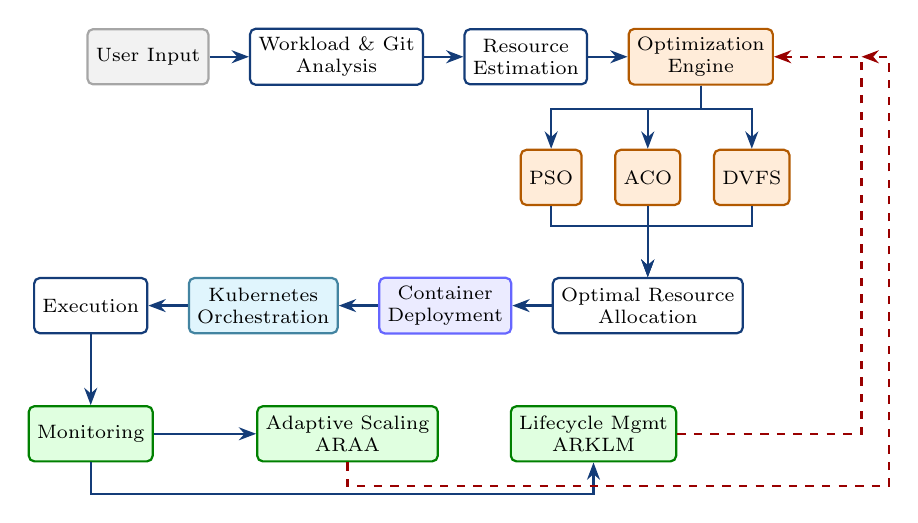
\begin{tikzpicture}[node distance=0.32cm and 0.5cm,
      every node/.style={font=\scriptsize}]
    % main column (horizontal layout to fit 16:9)
    \node[cli] (ui) {User Input};
    \node[box,right=of ui] (wl) {Workload \& Git\\Analysis};
    \node[box,right=of wl] (re) {Resource\\Estimation};
    \node[opt,right=of re] (oe) {Optimization\\Engine};

    \node[opt,below=0.8cm of oe,xshift=-1.9cm] (pso) {PSO};
    \node[opt,right=0.4cm of pso] (aco) {ACO};
    \node[opt,right=0.4cm of aco] (dvfs) {DVFS};

    \node[box,below=0.9cm of aco] (ora) {Optimal Resource\\Allocation};
    \node[dock,left=of ora] (cd) {Container\\Deployment};
    \node[k8s,left=of cd] (ko) {Kubernetes\\Orchestration};
    \node[box,left=of ko] (ex) {Execution};

    \node[mon,below=0.9cm of ex] (mo) {Monitoring};
    \node[mon,right=1.3cm of mo] (araa) {Adaptive Scaling\\ARAA};
    \node[mon,right=0.9cm of araa] (arklm) {Lifecycle Mgmt\\ARKLM};

    \draw[arr] (ui)--(wl); \draw[arr] (wl)--(re); \draw[arr] (re)--(oe);
    \draw[arr] (oe.south)--++(0,-0.3)-|(pso.north);
    \draw[arr] (oe.south)--++(0,-0.3)-|(aco.north);
    \draw[arr] (oe.south)--++(0,-0.3)-|(dvfs.north);
    \draw[arr] (pso.south)--++(0,-0.25)-|(ora.north);
    \draw[arr] (aco.south)--(ora.north);
    \draw[arr] (dvfs.south)--++(0,-0.25)-|(ora.north);
    \draw[arr] (ora)--(cd); \draw[arr] (cd)--(ko); \draw[arr] (ko)--(ex);
    \draw[arr] (ex)--(mo);
    \draw[arr] (mo)--(araa); \draw[arr] (mo.south)--++(0,-0.4)-|(arklm.south);
    % feedback
    \coordinate (fbx) at ($(dvfs.east)+(0.9,0)$);
    \draw[darr] (arklm.east) -- (arklm.east -| fbx) -- (fbx |- oe.east) -- (oe.east);
    \draw[darr] (araa.south) -- ++(0,-0.3) coordinate (fb2) -- (fb2 -| {$(fbx)+(0.35,0)$}) -- ({$(fbx)+(0.35,0)$} |- oe.east) -- ++(-0.35,0);
  \end{tikzpicture}

  \vspace{0.3em}
  {\scriptsize Dashed red arrows: closed-loop feedback to the Optimization Engine.}
\end{frame}

% ---------------- 8. Resource Utilization ----------------
\begin{frame}{Resource Utilization}
  \begin{itemize}
    \item Efficient use of computational resources such as CPU, memory, storage, and network in cloud environments.
    \item Demand varies dynamically due to:
      \begin{itemize}
        \item Multiple concurrent users
        \item Code execution workloads
        \item Real-time collaboration activities
      \end{itemize}
    \item Goal: maximize utilization while minimizing wastage and energy consumption.
    \item The system adopts an adaptive, optimization-driven resource utilization model.
  \end{itemize}
\end{frame}

% ---------------- 9. Types of Resources ----------------
\begin{frame}{Types of Resources Managed}
  \begin{description}
    \item[CPU Resources] Required for code execution, compilation, and processing
    \item[Memory (RAM)] Used for runtime environments and active sessions
    \item[Storage] Code files, logs, and container images
    \item[Network Bandwidth] Real-time collaboration and data transfer
    \item[Container Resources] Isolated execution environments for each user
  \end{description}
\end{frame}

% ---------------- 10. Optimization ----------------
\begin{frame}{Optimization-Based Utilization}
  \begin{columns}[T]
    \begin{column}{0.55\textwidth}
      \begin{itemize}
        \item \textbf{PSO} (Particle Swarm Optimization): finds optimal allocation of CPU and memory
        \item \textbf{ACO} (Ant Colony Optimization): efficient task scheduling across nodes
        \item \textbf{DVFS}: adjusts CPU power based on workload
      \end{itemize}
    \end{column}
    \begin{column}{0.4\textwidth}
      \begin{block}{Combined approach ensures}
        \begin{itemize}
          \item Balanced load distribution
          \item Reduced energy consumption
        \end{itemize}
      \end{block}
    \end{column}
  \end{columns}
\end{frame}

% ---------------- 11. FULL ARCHITECTURE ----------------
\begin{frame}[plain]
  \centering
  {\color{aitblue}\normalsize\bfseries System Architecture: Resource-Aware Collaborative Cloud IDE on Kubernetes}\\[-0.2em]
  \resizebox{\textwidth}{!}{%
  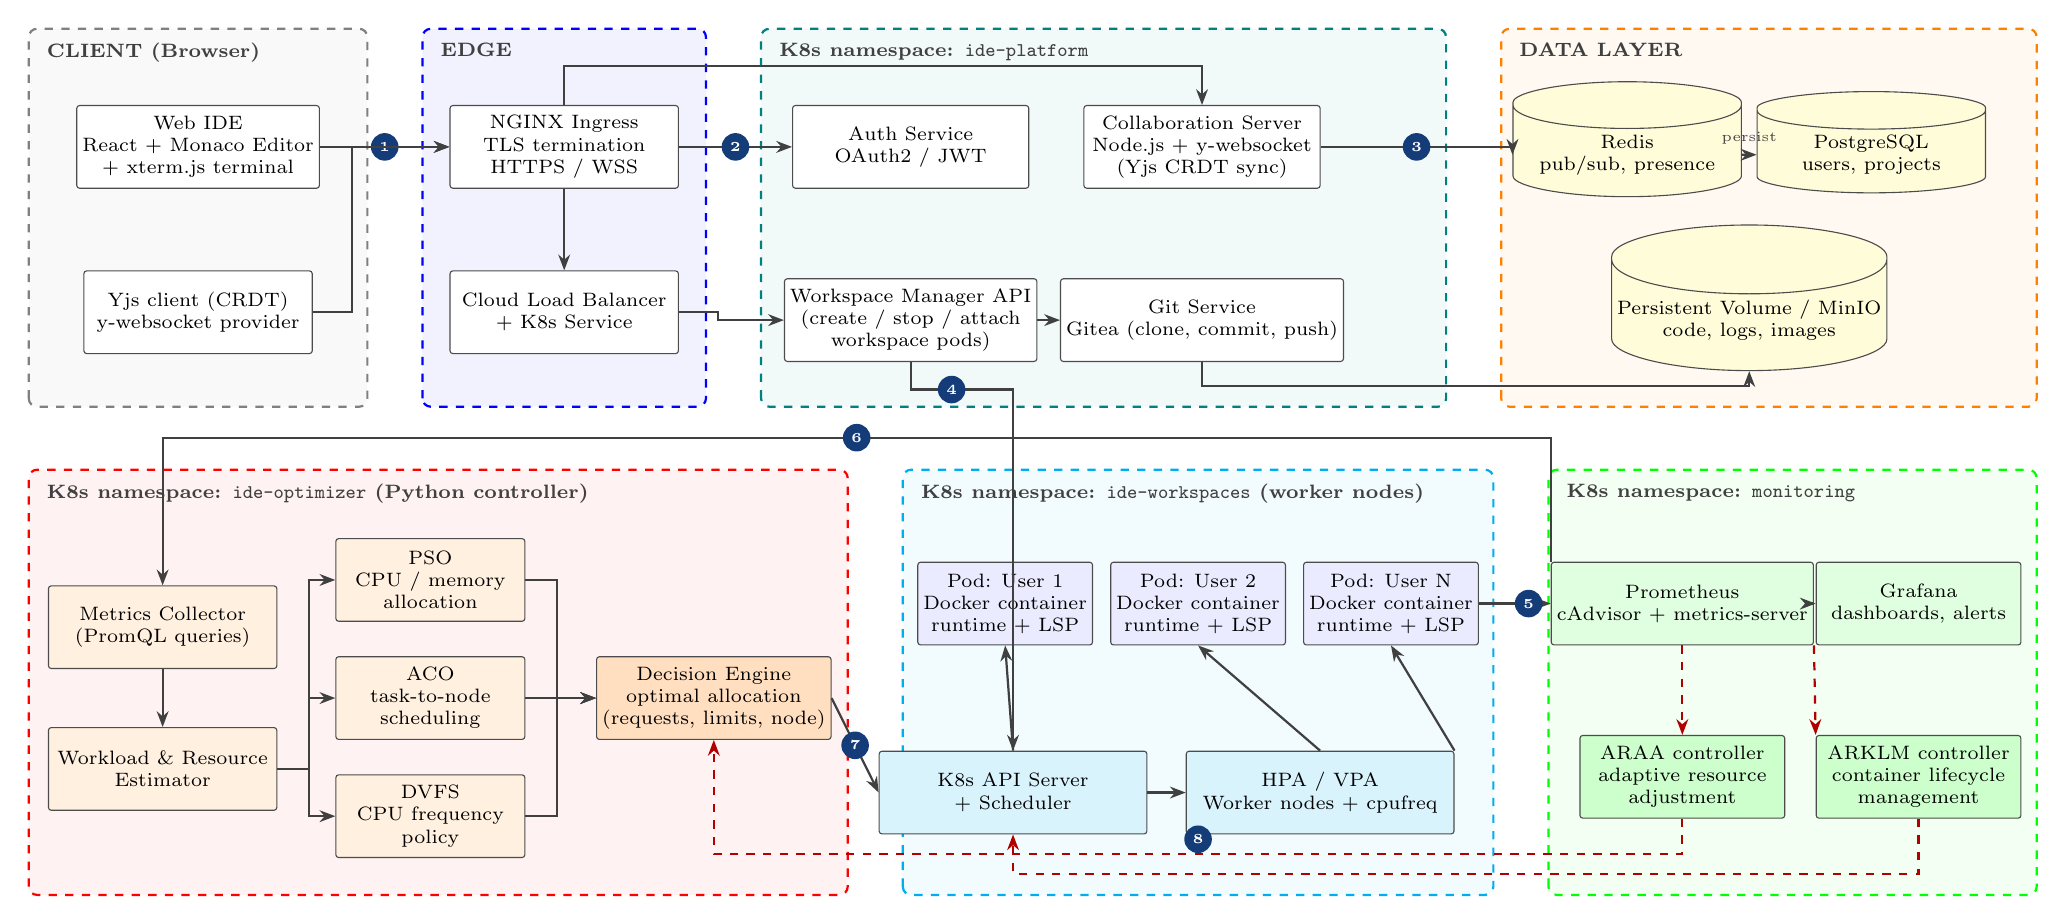
\begin{tikzpicture}[x=1cm,y=1cm,
     n/.style={draw=black!70,fill=white,rounded corners=1pt,minimum width=2.9cm,minimum height=1.05cm,align=center,font=\scriptsize,inner sep=2pt},
     nw/.style={n,minimum width=3.0cm},
     db/.style={n,cylinder,shape border rotate=90,aspect=0.25,fill=yellow!15,minimum height=1.2cm},
     gl/.style={font=\scriptsize\bfseries,anchor=north west,text=black!75},
     f/.style={-{Stealth[length=2mm]},thick,black!75},
     fb/.style={-{Stealth[length=2mm]},thick,dashed,red!70!black},
     num/.style={circle,fill=aitblue,text=white,font=\tiny\bfseries,inner sep=1pt,minimum size=3.5mm}]

  % ======= GROUPS =======
  \draw[g=gray]   (0,6.2) rectangle (4.3,11)    node[gl] at (0.1,10.95){CLIENT (Browser)};
  \draw[g=blue]   (5,6.2) rectangle (8.6,11)    node[gl] at (5.1,10.95){EDGE};
  \draw[g=teal]   (9.3,6.2) rectangle (18,11)   node[gl] at (9.4,10.95){K8s namespace: \texttt{ide-platform}};
  \draw[g=orange] (18.7,6.2) rectangle (25.5,11) node[gl] at (18.8,10.95){DATA LAYER};
  \draw[g=red]    (0,0) rectangle (10.4,5.4)    node[gl] at (0.1,5.35){K8s namespace: \texttt{ide-optimizer} (Python controller)};
  \draw[g=cyan]   (11.1,0) rectangle (18.6,5.4) node[gl] at (11.2,5.35){K8s namespace: \texttt{ide-workspaces} (worker nodes)};
  \draw[g=green]  (19.3,0) rectangle (25.5,5.4) node[gl] at (19.4,5.35){K8s namespace: \texttt{monitoring}};

  % ======= CLIENT =======
  \node[n] (br)  at (2.15,9.5) {Web IDE\\React + Monaco Editor\\+ xterm.js terminal};
  \node[n] (yc)  at (2.15,7.4) {Yjs client (CRDT)\\y-websocket provider};

  % ======= EDGE =======
  \node[n] (ing) at (6.8,9.5) {NGINX Ingress\\TLS termination\\HTTPS / WSS};
  \node[n] (lb)  at (6.8,7.4) {Cloud Load Balancer\\+ K8s Service};

  % ======= PLATFORM =======
  \node[nw] (auth) at (11.2,9.5)  {Auth Service\\OAuth2 / JWT};
  \node[nw] (col)  at (14.9,9.5)  {Collaboration Server\\Node.js + y-websocket\\(Yjs CRDT sync)};
  \node[nw] (wm)   at (11.2,7.3)  {Workspace Manager API\\(create / stop / attach\\workspace pods)};
  \node[nw] (git)  at (14.9,7.3)  {Git Service\\Gitea (clone, commit, push)};

  % ======= DATA =======
  \node[db] (red) at (20.3,9.4) {Redis\\pub/sub, presence};
  \node[db] (pg)  at (23.4,9.4) {PostgreSQL\\users, projects};
  \node[db] (pv)  at (21.85,7.3) {Persistent Volume / MinIO\\code, logs, images};

  % ======= OPTIMIZER =======
  \node[n,fill=orange!12] (mc)  at (1.7,3.4)  {Metrics Collector\\(PromQL queries)};
  \node[n,fill=orange!12] (est) at (1.7,1.6)  {Workload \& Resource\\Estimator};
  \node[n,fill=orange!12,minimum width=2.4cm] (pso) at (5.1,4.0) {PSO\\CPU / memory\\allocation};
  \node[n,fill=orange!12,minimum width=2.4cm] (aco) at (5.1,2.5) {ACO\\task-to-node\\scheduling};
  \node[n,fill=orange!12,minimum width=2.4cm] (dv)  at (5.1,1.0) {DVFS\\CPU frequency\\policy};
  \node[n,fill=orange!25,minimum width=2.6cm] (de)  at (8.7,2.5) {Decision Engine\\optimal allocation\\(requests, limits, node)};

  % ======= WORKSPACES =======
  \node[n,fill=blue!8,minimum width=2.1cm] (p1) at (12.4,3.7) {Pod: User 1\\Docker container\\runtime + LSP};
  \node[n,fill=blue!8,minimum width=2.1cm] (p2) at (14.85,3.7) {Pod: User 2\\Docker container\\runtime + LSP};
  \node[n,fill=blue!8,minimum width=2.1cm] (pn) at (17.3,3.7) {Pod: User N\\Docker container\\runtime + LSP};
  \node[n,fill=cyan!15,minimum width=3.4cm] (api) at (12.5,1.3) {K8s API Server\\+ Scheduler};
  \node[n,fill=cyan!15,minimum width=3.4cm] (hpa) at (16.4,1.3) {HPA / VPA\\Worker nodes + cpufreq};

  % ======= MONITORING =======
  \node[n,fill=green!12,minimum width=2.6cm] (prom) at (21.0,3.7) {Prometheus\\cAdvisor + metrics-server};
  \node[n,fill=green!12,minimum width=2.6cm] (graf) at (24.0,3.7) {Grafana\\dashboards, alerts};
  \node[n,fill=green!20,minimum width=2.6cm] (araa) at (21.0,1.5) {ARAA controller\\adaptive resource\\adjustment};
  \node[n,fill=green!20,minimum width=2.6cm] (arklm) at (24.0,1.5) {ARKLM controller\\container lifecycle\\management};

  % ======= FLOWS =======
  \draw[f] (br) -- node[num,pos=0.5]{1} (ing);
  \draw[f] (yc.east) -- ++(0.5,0) |- (ing.west);
  \draw[f] (ing) -- (lb);
  \draw[f] (ing.east) -- node[num,pos=0.5]{2} (auth.west);
  \draw[f] (lb.east) -- ++(0.5,0) |- (wm.west);
  \draw[f] (ing.north) -- ++(0,0.5) -| (col.north);
  \draw[f] (col) -- node[num]{3} (red.west |- col.east) -- (red.west);
  \draw[f] (wm) -- (git);
  \draw[f] (git.south) -- ++(0,-0.3) -| (pv.south);
  \draw[f,dashed] (red.east) -- node[above,font=\tiny]{persist} (pg.west);

  % workspace creation
  \draw[f] (wm.south) -- ++(0,-0.35) -| node[num,pos=0.2]{4} (api.north);
  \draw[f] (api.north) -- (p1.south);
  \draw[f] (api.east) -- (hpa.west);
  \draw[f] (hpa.north) -- (p2.south);
  \draw[f] (hpa.north east) -- (pn.south);

  % metrics path
  \draw[f] (pn.east) -- ++(0.35,0) |- node[num,pos=0.75]{5} (prom.west);
  \draw[f] (prom.north west) -- ++(0,1.575) -| node[num,pos=0.25]{6} (mc.north);
  \draw[f] (prom) -- (graf);

  % optimization pipeline
  \draw[f] (mc) -- (est);
  \draw[f] (est.east) -- ++(0.4,0) |- (pso.west);
  \draw[f] (est.east) -- ++(0.4,0) |- (aco.west);
  \draw[f] (est.east) -- ++(0.4,0) |- (dv.west);
  \draw[f] (pso.east) -- ++(0.4,0) |- (de.west);
  \draw[f] (aco.east) -- (de.west);
  \draw[f] (dv.east) -- ++(0.4,0) |- (de.west);
  \draw[f] (de.east) -- node[num,pos=0.5]{7} (api.west);

  % feedback loop (MAPE-K)
  \draw[fb] (prom.south) -- (araa.north);
  \draw[fb] (prom.south east) -- (arklm.north west);
  \draw[fb] (araa.south) -- ++(0,-0.45) -| (de.south) node[num,pos=0.25,above]{8};
  \draw[fb] (arklm.south) -- ++(0,-0.7) -| (api.south);
  \end{tikzpicture}}

  \par\vspace{0.4em}
  \tiny
  \textbf{Flows:}
  1~HTTPS/WSS from browser \quad 2~route to Auth, Collab, Workspace API \quad 3~CRDT updates via Redis pub/sub, state in PostgreSQL \quad 4~Workspace Manager asks K8s API to create a user pod \quad 5~pod metrics scraped by Prometheus \quad 6~Metrics Collector queries Prometheus \quad 7~Decision Engine patches requests/limits and node placement; DVFS sets CPU frequency \quad 8~ARAA/ARKLM feedback (MAPE-K loop, dashed).
\end{frame}

% ---------------- 12. Conclusion ----------------
\begin{frame}{Conclusion}
  \begin{itemize}
    \item Real-time collaborative coding in the cloud using \textbf{Docker} for isolated environments and \textbf{Kubernetes} for scalability and load balancing.
    \item Intelligent optimization (PSO, ACO, DVFS) improves resource utilization and performance, enabling multiple users to work efficiently with low latency.
    \item Ensures reliability, scalability, and enhanced developer productivity, making it a modern and future-ready cloud IDE solution.
  \end{itemize}
  \vfill
  \centering\Large\color{aitblue}Thank You
\end{frame}

\end{document}